\clearpage

\section{Results in the ee and $\mu\mu$ Channels}
\label{app:results}

In this section we provide the results of the inclusive and targeted searches, separately in the ee and $\mu\mu$ channels.
The \MET\ distributions in the inclusive analysis for the ee channel are displayed in Fig.~\ref{fig:results_incl_ee} and 
the signal region yields are presented in Table~\ref{tab:results_incl_ee}.
The \MET\ distributions in the inclusive analysis for the $\mu\mu$ channel are displayed in Fig.~\ref{fig:results_incl_mm} and 
the signal region yields are presented in Table~\ref{tab:results_incl_mm}.

\begin{figure}[!h]
\begin{center}
\begin{tabular}{cc}
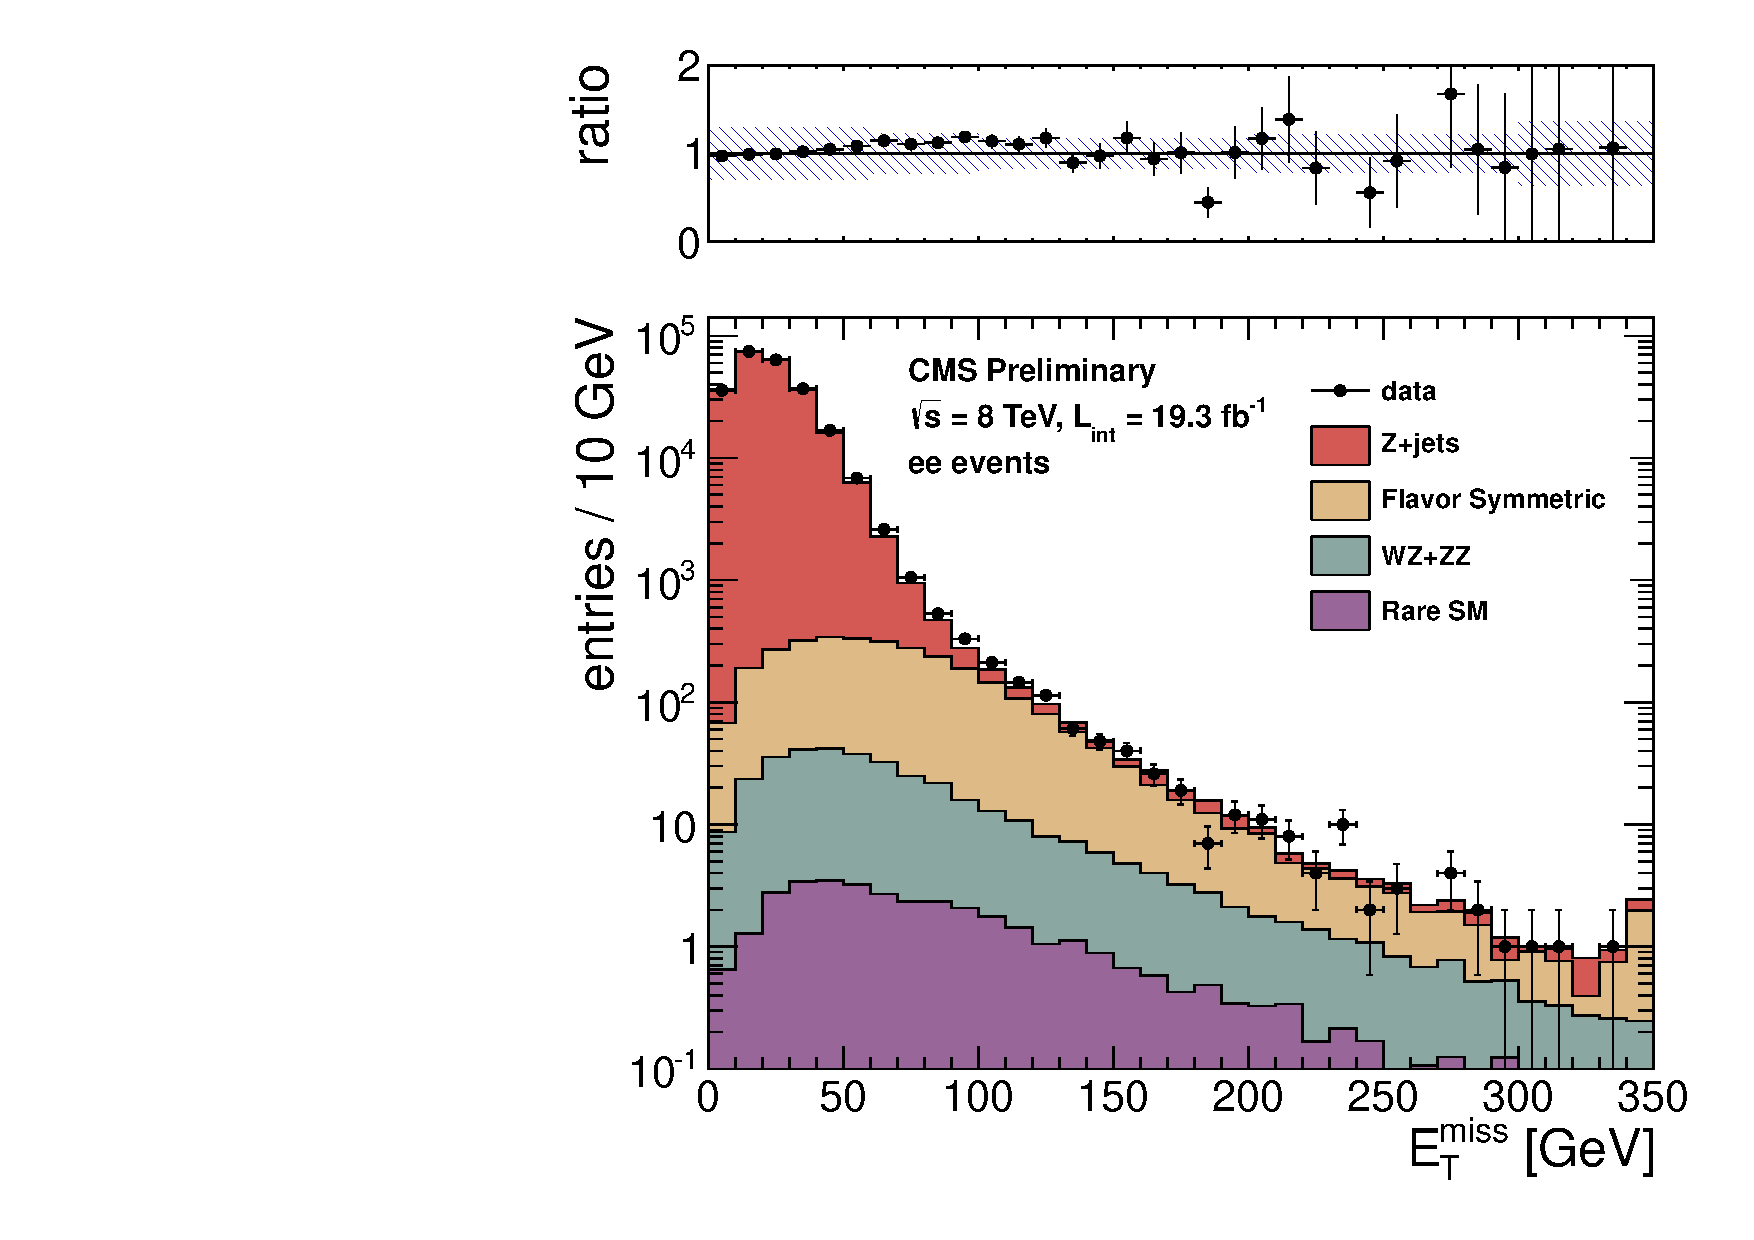
\includegraphics[width=0.6\textwidth]{plots/pfmet_ee_19fb.pdf}
\end{tabular}
\caption{Results of the inclusive analysis in the ee channel. The observed \MET\ distribution (black points) is compared with the sum of the predicted \MET\
distributions from \zjets, flavor-symmetric backgrounds, and WZ+ZZ backgrounds. The ratio of observed to predicted yields in each bin is
indicated. The error bars indicate the statistical uncertainty in the data and the shaded band indicates the total background uncertainty.
\label{fig:results_incl_ee}
}
\end{center}
\end{figure}

\begin{table}[htb]
\begin{center}
\footnotesize
\caption{\label{tab:results_incl_ee} Summary of results in the inclusive analysis in the ee channel. The total background is the sum of the \zjets\ background predicted from
the \MET\ templates method (\zjets\ bkg), the flavor-symmetric background predicted from e$\mu$ events (FS bkg), and the WZ and ZZ backgrounds predicted from MC
(WZ bkg and ZZ bkg). All uncertainties include both the statistical and systematic components. The Gaussian significance of the deviation between the data 
and total background is indicated for signal regions with at least 20 observed events. }
\begin{tabular}{l|c|c|c|c|c|c}

\hline
\hline

\begin{comment}
ee channel: scale em yield by 0.44
Yields in 0-60 GeV region
data   : 234412
gjets  : 236535
OF     : 1337.64
WZ     : 152.474
ZZ     : 21.4167
Rare   : 14.846
Scaling gjets by : 0.984573
SF events 239661
OF events 44581
\end{comment}

                      &   \MET\ 0--30 GeV   &  \MET\ 30--60 GeV   & \MET\ 60--100 GeV   &\MET\ 100--200 GeV   &\MET\ 200--300 GeV   & \MET\ $>$ 300 GeV  \\
        \zjets\ bkg   &175315 $\pm$ 52599   & 57571 $\pm$ 17279   &    2957 $\pm$ 900   &      120 $\pm$ 58   &     5.5 $\pm$ 1.7   &     1.3 $\pm$ 0.5  \\
             FS bkg   &      463 $\pm$ 87   &     875 $\pm$ 163   &     923 $\pm$ 172   &      459 $\pm$ 86   &    22.9 $\pm$ 7.2   &     3.3 $\pm$ 2.0  \\
             WZ bkg   &   56.5 $\pm$ 39.6   &   95.9 $\pm$ 67.2   &   70.1 $\pm$ 49.1   &   38.3 $\pm$ 26.8   &     5.4 $\pm$ 3.8   &     1.6 $\pm$ 1.6  \\
             ZZ bkg   &     6.9 $\pm$ 3.4   &    14.6 $\pm$ 7.3   &    15.6 $\pm$ 7.8   &    14.6 $\pm$ 7.3   &     3.2 $\pm$ 1.6   &     0.8 $\pm$ 0.8  \\
        rare SM bkg   &     4.7 $\pm$ 2.4   &    10.1 $\pm$ 5.1   &     9.5 $\pm$ 4.7   &     8.8 $\pm$ 4.4   &     1.8 $\pm$ 0.9   &     0.6 $\pm$ 0.6  \\
          total bkg   &175846 $\pm$ 52599   & 58566 $\pm$ 17280   &    3975 $\pm$ 918   &     641 $\pm$ 108   &    38.7 $\pm$ 8.5   &     7.7 $\pm$ 2.8  \\
               data   &            173814   &             60598   &              4516   &               685   &                45   &                 3  \\
       significance   &      -0.0$\sigma$   &       0.1$\sigma$   &       0.6$\sigma$   &       0.4$\sigma$   &       0.6$\sigma$   &      -1.4$\sigma$  \\

\hline
\hline
\end{tabular}
\end{center}
\end{table}

\clearpage

\begin{figure}[!h]
\begin{center}
\begin{tabular}{cc}
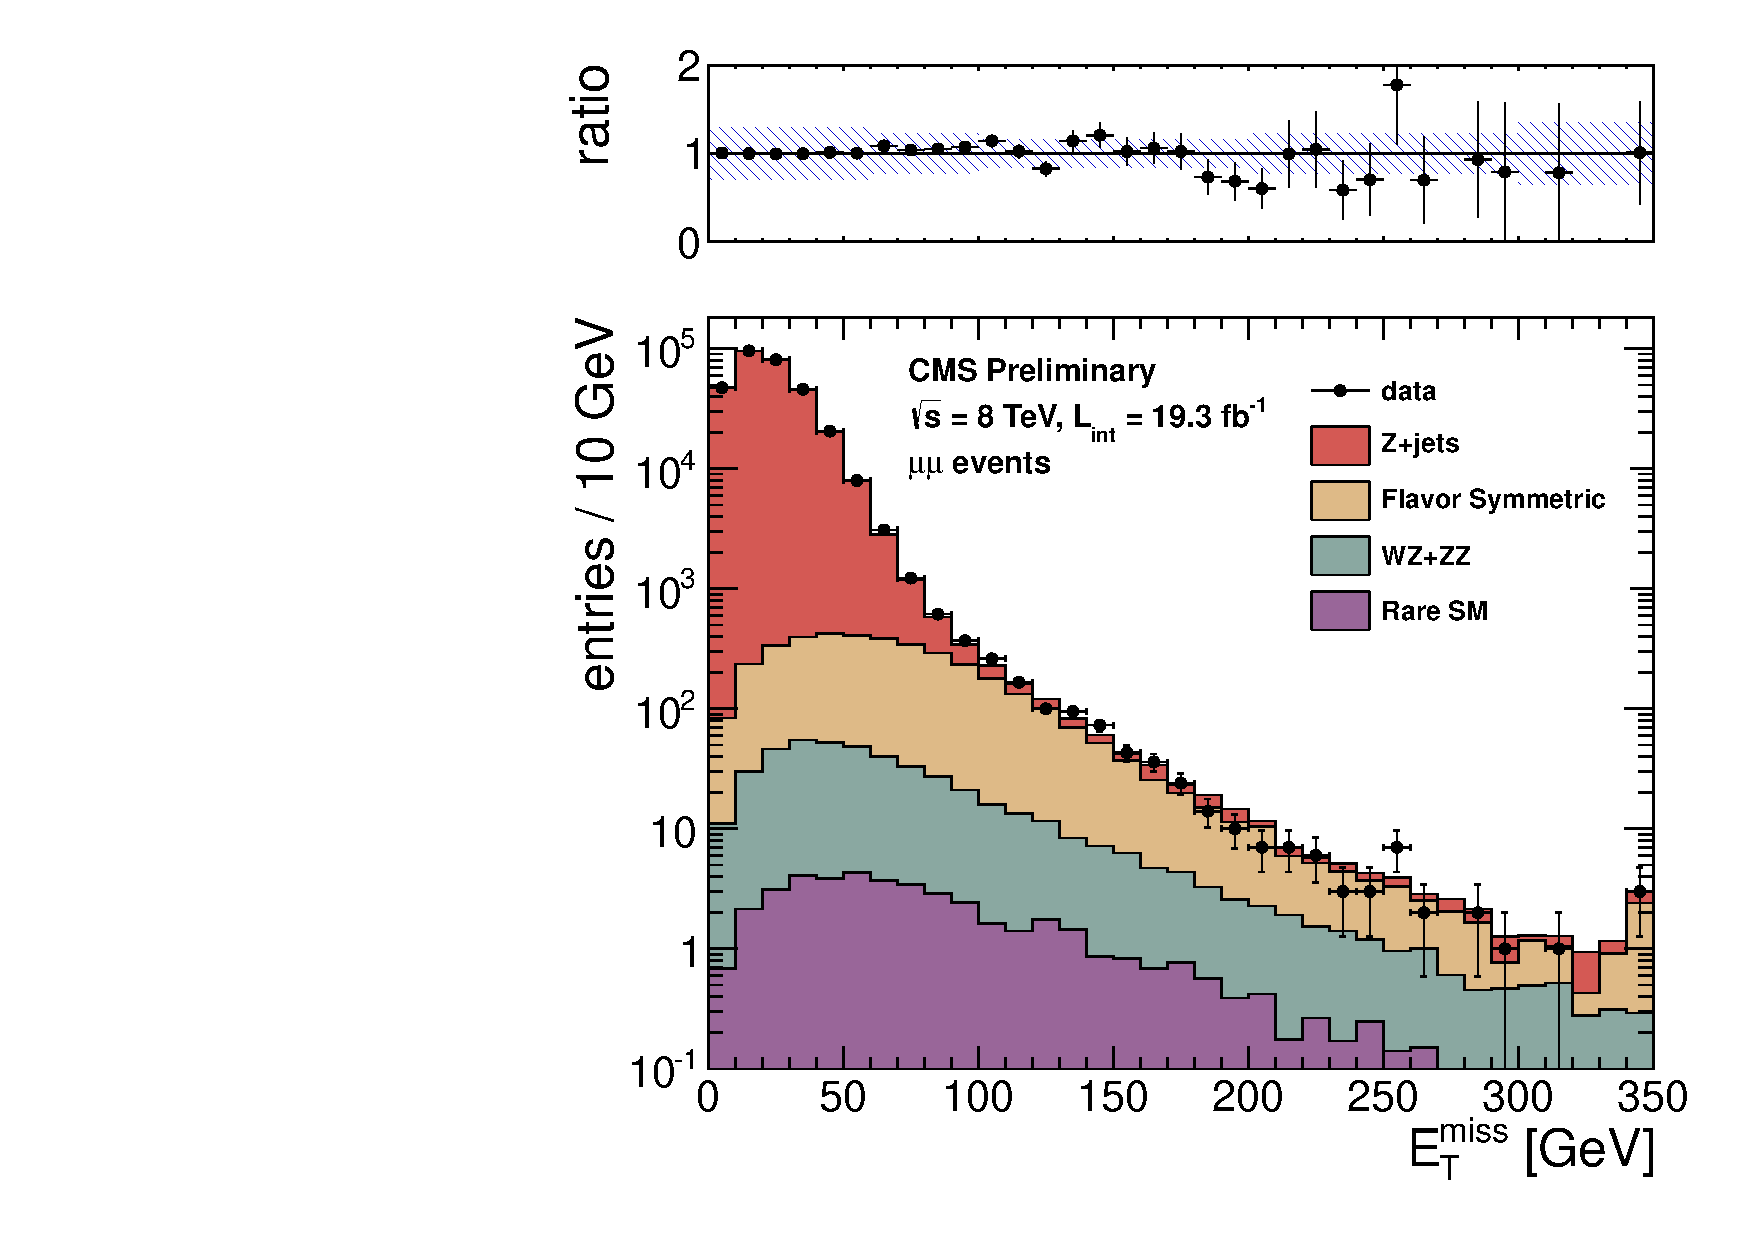
\includegraphics[width=0.6\textwidth]{plots/pfmet_mm_19fb.pdf}
\end{tabular}
\caption{Results of the inclusive analysis in the $\mu\mu$ channel. The observed \MET\ distribution (black points) is compared with the sum of the predicted \MET\
distributions from \zjets, flavor-symmetric backgrounds, and WZ+ZZ backgrounds. The ratio of observed to predicted yields in each bin is
indicated. The error bars indicate the statistical uncertainty in the data and the shaded band indicates the total background uncertainty.
\label{fig:results_incl_mm}
}
\end{center}
\end{figure}

\begin{table}[htb]
\begin{center}
\footnotesize
\caption{\label{tab:results_incl_mm} Summary of results in the inclusive analysis in the $\mu\mu$ channel. The total background is the sum of the \zjets\ background predicted from
the \MET\ templates method (\zjets\ bkg), the flavor-symmetric background predicted from e$\mu$ events (FS bkg), and the WZ and ZZ backgrounds predicted from MC
(WZ bkg and ZZ bkg). All uncertainties include both the statistical and systematic components. The Gaussian significance of the deviation between the data 
and total background is indicated for signal regions with at least 20 observed events. }
\begin{tabular}{l|c|c|c|c|c|c}

\hline
\hline

\begin{comment}
mm channel: scale em yield by 0.54
Yields in 0-60 GeV region
data   : 298789
gjets  : 301055
OF     : 1641.65
WZ     : 196.298
ZZ     : 28.4562
Rare   : 18.2493
Scaling gjets by : 0.986214
SF events 304953
OF events 44581
\end{comment}

                      &   \MET\ 0--30 GeV   &  \MET\ 30--60 GeV   & \MET\ 60--100 GeV   &\MET\ 100--200 GeV   &\MET\ 200--300 GeV   & \MET\ $>$ 300 GeV  \\
        \zjets\ bkg   &223877 $\pm$ 67165   & 73027 $\pm$ 21910   &   3694 $\pm$ 1111   &      146 $\pm$ 50   &     6.7 $\pm$ 2.1   &     1.7 $\pm$ 0.6  \\
             FS bkg   &     568 $\pm$ 106   &    1074 $\pm$ 201   &    1133 $\pm$ 212   &     563 $\pm$ 105   &    28.1 $\pm$ 8.8   &     4.1 $\pm$ 2.4  \\
             WZ bkg   &   72.4 $\pm$ 50.7   &  123.9 $\pm$ 86.7   &   88.1 $\pm$ 61.7   &   48.1 $\pm$ 33.7   &     6.5 $\pm$ 4.5   &     1.6 $\pm$ 1.6  \\
             ZZ bkg   &     9.1 $\pm$ 4.5   &    19.4 $\pm$ 9.7   &   20.9 $\pm$ 10.5   &    19.2 $\pm$ 9.6   &     3.6 $\pm$ 1.8   &     1.2 $\pm$ 1.2  \\
        rare SM bkg   &     6.0 $\pm$ 3.0   &    12.3 $\pm$ 6.2   &    12.4 $\pm$ 6.2   &    10.3 $\pm$ 5.2   &     1.8 $\pm$ 0.9   &     0.7 $\pm$ 0.7  \\
          total bkg   &224532 $\pm$ 67165   & 74257 $\pm$ 21911   &   4948 $\pm$ 1133   &     787 $\pm$ 122   &   46.6 $\pm$ 10.3   &     9.2 $\pm$ 3.3  \\
               data   &            224334   &             74455   &              5300   &               822   &                38   &                 4  \\
       significance   &      -0.0$\sigma$   &       0.0$\sigma$   &       0.3$\sigma$   &       0.3$\sigma$   &      -0.7$\sigma$   &      -1.4$\sigma$  \\

\hline
\hline
\end{tabular}
\end{center}
\end{table}


\clearpage

The \MET\ distributions in the targeted analysis for the ee channel are displayed in Fig.~\ref{fig:results_targ_ee} and 
the signal region yields are presented in Table~\ref{tab:results_targ_ee}.
The \MET\ distributions in the inclusive analysis for the $\mu\mu$ channel are displayed in Fig.~\ref{fig:results_targ_mm} and 
the signal region yields are presented in Table~\ref{tab:results_targ_mm}.

\begin{figure}[!h]
\begin{center}
\begin{tabular}{cc}
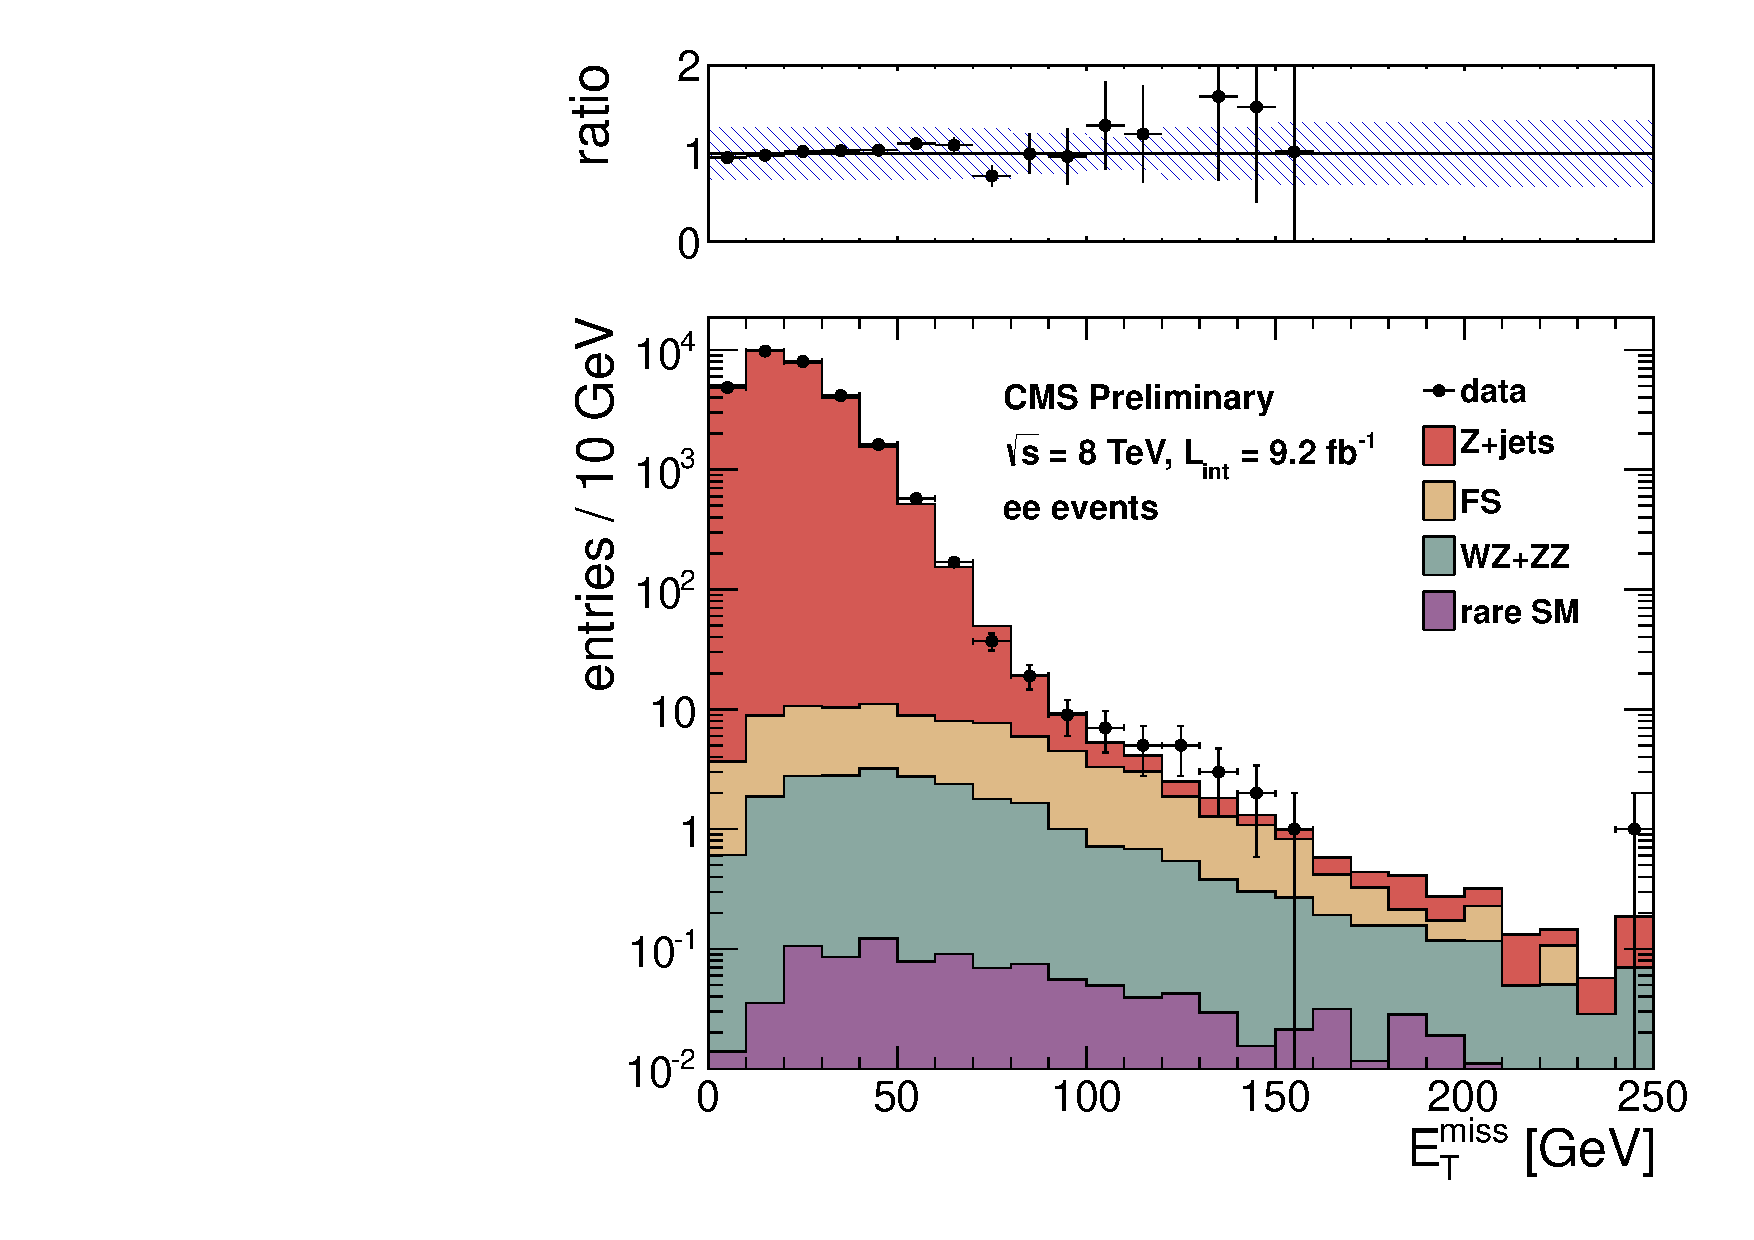
\includegraphics[width=0.5\textwidth]{plots/pfmet_bvetoMedium_ee.pdf}
\end{tabular}
\caption{Results of the targeted analysis in the ee channel. The observed \MET\ distribution (black points) is compared with the sum of the predicted \MET\
distributions from \zjets, flavor-symmetric backgrounds, and WZ+ZZ backgrounds. The ratio of observed to predicted yields in each bin is
indicated. The error bars indicate the statistical uncertainty in the data and the shaded band indicates the total background uncertainty.
\label{fig:results_targ_ee}
}
\end{center}
\end{figure}



\begin{table}[htb]
\begin{center}
\footnotesize
\caption{\label{tab:results_targ_ee}\footnotesize Summary of results in the targeted analysis in the ee channel. The total background is the sum of the \zjets\ background predicted from
the \MET\ templates method (\zjets\ bkg), the flavor-symmetric background predicted from e$\mu$ events (FS bkg), and the WZ and ZZ backgrounds predicted from MC
(WZ bkg and ZZ bkg). All uncertainties include both the statistical and systematic components. The Gaussian significance of the deviation between the data 
and total background is indicated for signal regions with at least 20 observed events. }
\begin{tabular}{l|c|c|c|c}

\hline
\hline

\begin{comment}
ee channel: scale em yield by 0.43
Yields in 0-60 GeV region
data   : 28925
gjets  : 28970.5
OF     : 39.4654
WZ     : 10.9283
ZZ     : 2.66597
Rare   : 0.442106
Scaling gjets by : 0.996582
SF events 29183
OF events 1214

ee events
\end{comment}

                      &   \MET\ 0--30 GeV   &  \MET\ 30--60 GeV   &  \MET\ 60--80 GeV   & \MET\ 80--100 GeV   \\
\hline
        \zjets\ bkg   &  22806 $\pm$ 6842   &   6065 $\pm$ 1820   &      188 $\pm$ 57   &    17.9 $\pm$ 6.2   \\
             FS bkg   &    17.9 $\pm$ 3.6   &    21.5 $\pm$ 4.3   &    11.5 $\pm$ 2.4   &     7.8 $\pm$ 1.7   \\
             WZ bkg   &     4.2 $\pm$ 2.9   &     6.8 $\pm$ 4.7   &     3.0 $\pm$ 2.1   &     1.8 $\pm$ 1.2   \\
             ZZ bkg   &     1.0 $\pm$ 0.5   &     1.7 $\pm$ 0.9   &     1.0 $\pm$ 0.5   &     0.8 $\pm$ 0.4   \\
        rare SM bkg   &     0.2 $\pm$ 0.1   &     0.3 $\pm$ 0.1   &     0.2 $\pm$ 0.1   &     0.1 $\pm$ 0.1   \\
\hline
          total bkg   &  22830 $\pm$ 6842   &   6095 $\pm$ 1820   &      204 $\pm$ 58   &    28.4 $\pm$ 6.5   \\
               data   &             22581   &              6344   &               206   &                28   \\
       significance   &      -0.0$\sigma$   &       0.1$\sigma$   &       0.0$\sigma$   &      -0.0$\sigma$   \\
\hline
\hline
                      &\MET\ 100--120 GeV   &\MET\ 120--150 GeV   &\MET\ 150--200 GeV   & \MET\ $>$ 200 GeV  \\
\hline
        \zjets\ bkg   &     3.1 $\pm$ 1.1   &     1.4 $\pm$ 1.4   &     0.7 $\pm$ 0.7   &     0.4 $\pm$ 0.1  \\
             FS bkg   &     4.9 $\pm$ 1.1   &     3.0 $\pm$ 0.7   &     1.1 $\pm$ 0.5   &     0.2 $\pm$ 0.1  \\
             WZ bkg   &     0.9 $\pm$ 0.6   &     0.7 $\pm$ 0.5   &     0.4 $\pm$ 0.3   &     0.2 $\pm$ 0.2  \\
             ZZ bkg   &     0.4 $\pm$ 0.2   &     0.4 $\pm$ 0.2   &     0.4 $\pm$ 0.2   &     0.3 $\pm$ 0.3  \\
        rare SM bkg   &     0.1 $\pm$ 0.0   &     0.1 $\pm$ 0.0   &     0.1 $\pm$ 0.1   &     0.1 $\pm$ 0.1  \\
\hline
          total bkg   &     9.4 $\pm$ 1.7   &     5.6 $\pm$ 1.7   &     2.7 $\pm$ 0.9   &     1.1 $\pm$ 0.4  \\
               data   &                12   &                10   &                 1   &                 1  \\
       significance   &                     &                     &                     &                    \\


\hline
\hline

\end{tabular}
\end{center}
\end{table}


\clearpage

\begin{figure}[!h]
\begin{center}
\begin{tabular}{cc}
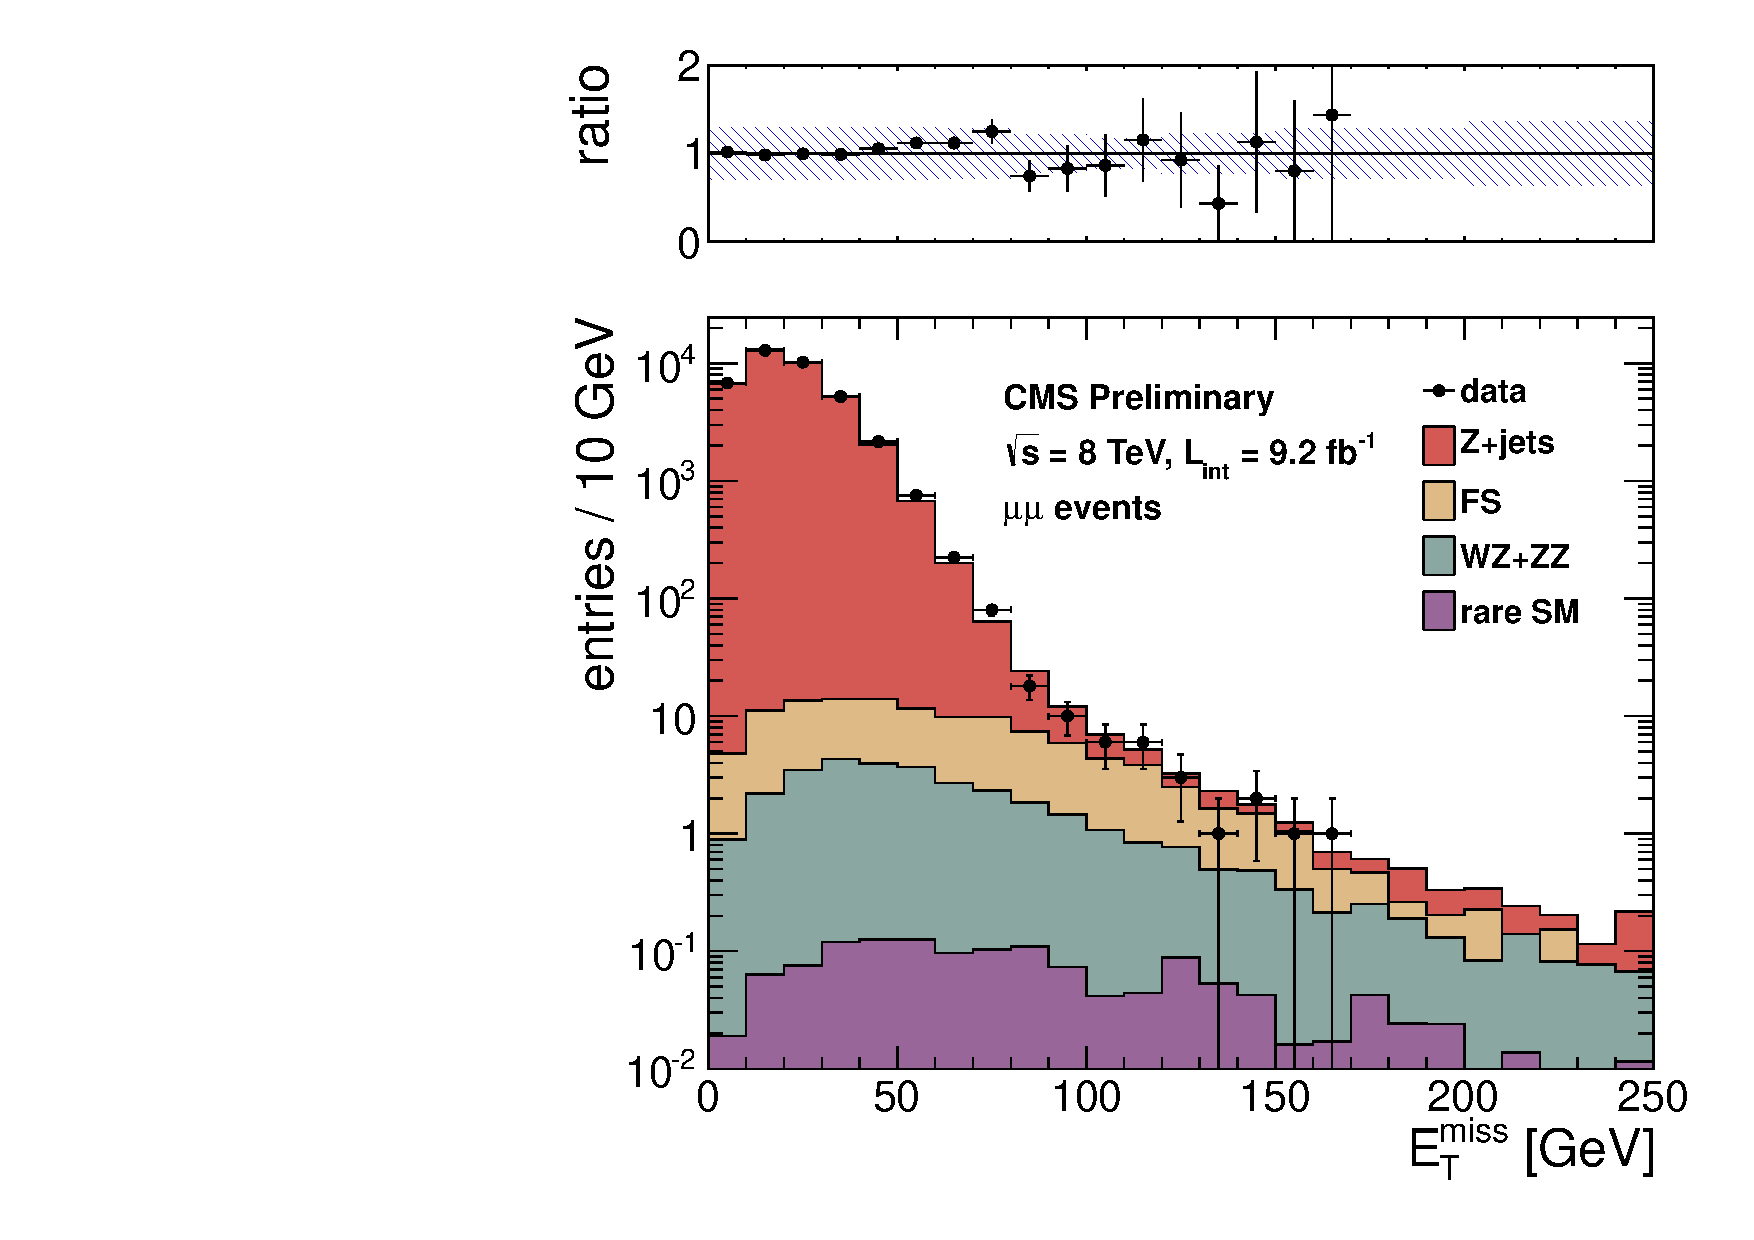
\includegraphics[width=0.5\textwidth]{plots/pfmet_bvetoMedium_mm.pdf}
\end{tabular}
\caption{Results of the targeted analysis in the $\mu\mu$ channel. The observed \MET\ distribution (black points) is compared with the sum of the predicted \MET\
distributions from \zjets, flavor-symmetric backgrounds, and WZ+ZZ backgrounds. The ratio of observed to predicted yields in each bin is
indicated. The error bars indicate the statistical uncertainty in the data and the shaded band indicates the total background uncertainty.
\label{fig:results_targ_mm}
}
\end{center}
\end{figure}



\begin{table}[htb]
\begin{center}
\footnotesize
\caption{\label{tab:results_targ_mm}\footnotesize Summary of results in the targeted analysis in the $\mu\mu$ channel. The total background is the sum of 
the \zjets\ background predicted from
the \MET\ templates method (\zjets\ bkg), the flavor-symmetric background predicted from e$\mu$ events (FS bkg), and the WZ and ZZ backgrounds predicted from MC
(WZ bkg and ZZ bkg). All uncertainties include both the statistical and systematic components. The Gaussian significance of the deviation between the data 
and total background is indicated for signal regions with at least 20 observed events. }
\begin{tabular}{l|c|c|c|c}

\hline
\hline


\begin{comment}
mm channel: scale em yield by 0.55
Yields in 0-60 GeV region
data   : 38036
gjets  : 38112.2
OF     : 50.479
WZ     : 14.4673
ZZ     : 3.52228
Rare   : 0.529845
Scaling gjets by : 0.996189
SF events 38388
OF events 1214

#mu#mu events
\end{comment}

                      &   \MET\ 0--30 GeV   &  \MET\ 30--60 GeV   &  \MET\ 60--80 GeV   & \MET\ 80--100 GeV   \\
\hline
        \zjets\ bkg   &  30017 $\pm$ 9005   &   7950 $\pm$ 2385   &      245 $\pm$ 74   &    23.0 $\pm$ 7.2   \\
             FS bkg   &    23.0 $\pm$ 4.7   &    27.5 $\pm$ 5.6   &    14.7 $\pm$ 3.0   &     9.9 $\pm$ 2.1   \\
             WZ bkg   &     5.3 $\pm$ 3.7   &     9.2 $\pm$ 6.4   &     3.6 $\pm$ 2.5   &     2.1 $\pm$ 1.5   \\
             ZZ bkg   &     1.1 $\pm$ 0.6   &     2.4 $\pm$ 1.2   &     1.2 $\pm$ 0.6   &     1.0 $\pm$ 0.5   \\
        rare SM bkg   &     0.2 $\pm$ 0.1   &     0.4 $\pm$ 0.2   &     0.2 $\pm$ 0.1   &     0.2 $\pm$ 0.1   \\
\hline
          total bkg   &  30046 $\pm$ 9005   &   7990 $\pm$ 2385   &      264 $\pm$ 74   &    36.2 $\pm$ 7.6   \\
               data   &             29904   &              8132   &               304   &                28   \\
       significance   &      -0.0$\sigma$   &       0.1$\sigma$   &       0.5$\sigma$   &      -0.9$\sigma$   \\

\hline
\hline

                      &\MET\ 100--120 GeV   &\MET\ 120--150 GeV   &\MET\ 150--200 GeV   & \MET\ $>$ 200 GeV  \\
\hline
        \zjets\ bkg   &     3.9 $\pm$ 1.2   &     1.7 $\pm$ 1.2   &     0.9 $\pm$ 0.6   &     0.5 $\pm$ 0.1  \\
             FS bkg   &     6.3 $\pm$ 1.4   &     3.9 $\pm$ 0.9   &     1.4 $\pm$ 0.6   &     0.2 $\pm$ 0.2  \\
             WZ bkg   &     1.2 $\pm$ 0.9   &     0.9 $\pm$ 0.6   &     0.6 $\pm$ 0.4   &     0.3 $\pm$ 0.3  \\
             ZZ bkg   &     0.6 $\pm$ 0.3   &     0.7 $\pm$ 0.4   &     0.4 $\pm$ 0.2   &     0.4 $\pm$ 0.4  \\
        rare SM bkg   &     0.1 $\pm$ 0.0   &     0.2 $\pm$ 0.1   &     0.1 $\pm$ 0.1   &     0.1 $\pm$ 0.1  \\
\hline
          total bkg   &    12.1 $\pm$ 2.1   &     7.3 $\pm$ 1.7   &     3.4 $\pm$ 1.0   &     1.4 $\pm$ 0.5  \\
               data   &                12   &                 6   &                 2   &                 0  \\
       significance   &                     &                     &                     &                    \\
\hline
\hline


\end{tabular}
\end{center}
\end{table}

